\section{$\lgname$ Software Stack}
\label{sec:software}

\subsection{Runtime system}
 The $\lgname$ runtime system comprises of a program which interacts with the controller plane through sensor and actuator ports, which in turn communicates with the physical plant through ROS messages. The software stack implementing this uses the $\lgname$ front-end, that takes as input a $\lgname$ program and generates a python program, that runs on a middle layer (written in python) on the agents in the system (either in simulation or on actual hardware). In actual deployment, python middle layer communicates through ROS messages with the ROS interfaces for the low level hardware controls. 

\begin{figure}[h!]
\centering
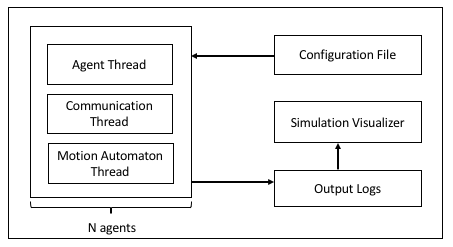
\includegraphics[width=0.48\textwidth]{figs/simulationengine.png}
\caption{Simulation of a $\lgname$ program }
\label{fig:simfig}
\end{figure}
The python middle layer in our implementation of the $\lgname$ language consists of the following major modules:\begin{inparaenum}
\item a communication module implementing the shared memory semantics,\item a motion module which in simulation implementing the dynamics of the environment, and in hardware, is responsible for publishing and subscribing to ROS messages between the program and the platform. \item an agent thread module which implements the discrete event loop semantics of each agent. 
\end{inparaenum}. To run a $\lgname$ program (hardware or simulation), the user has to provide a configuration file, with \begin{inparaenum}\item the number of agents, \item in case of simulation, the initial positions of the agents and the length of the simulation and \item in case of hardware deployment their IP addresses, and the localization system.\end{inparaenum} Each agent in the system launches the agent thread, which has its own \emph{Motion automaton} thread, which implements the controller for the agent thread. Each agent thread also has a communication thread, which it uses to listen for and send messages for shared variable updates to other agent threads. In simulation, the $\lgname$ program launches $N$ threads, each with its own communication and motion automaton threads, and runs the execution as long as specified in the program.


\paragraph{Addressing the gap between theory and implementation}

Usually cyber-physical system models are based on mathematical representations of the system without an emphasis on the implementability of said model. Our formal \emph{executable} semantics is intended to narrow that the gap between the theory and implementation of cyber-physical systems, as the translation of the mathematical rules into exact rewrite rules in the \K-semantic framework ensures that. Our python middle layer, which is used to run the $\lgname$ programs in simulation as well as on hardware relies on several assumptions, which we discuss in the next subsection.



\subsection{Key Assumptions} 

\paragraph*{Periodic event execution semantics}
 Our semantics assumes periodic execution of agent programs, with minimum period defined by the sampling parameter $\delta>0$. This is a standard programming style in embedded and control systems. Several other languages, such as Giotto~\cite{henzinger2003giotto}, use similar semantics. The Giotto paper shows how interrupts can be emulated in this execution model. One of the other assumptions is that the program transitions in a round have  zero logical execution time. In our implementation, the participating agents run barrier synchronization algorithms, and we ensure that the controller only starts driving the physical plant after the maximum possible time to execute a program transition step for each agent has elapsed. 


\paragraph*{Shared variable implementation through message passing}
For the shared memory abstraction to be faithfully implemented on a message-passing wireless network, the message delays between agents should be less than the the sampling parameter $\delta$. We use TCP/UDP to send agent shared variable update messages over Wifi in our implementation. The messages are propagated during the \emph{environment transition} in each round, and processed before the next round of program transitions starts.

\paragraph*{Portability and heterogeneity}

$\lgname$ programs are portable in the sense that the same application code, can be executed with different controller and plant (environment) executables that provide the same ports. We can execute most application with an environment which is either a model of a different type of wheeled robot or a quadcopter, or even the actual hardware platforms. 

The implementation of the $\lgname$ supports middle level path-planning module replacement in addition to lower level vehicle dynamics. The  choice of path planner  used  can  be  platform-specific  and/or  application-specific. We designed the $\lgname$ software stack in a modular fashion, to allow a user to implement any path planning strategies if a different motion behavior is desired. This allows for deployment of the same $\lgname$ program on different platforms as long as they support the same sensor and actuator ports. 

\paragraph*{Known set of participants}
Current design and implementation of $\lgname$ builds on the assumption that the number and identities of the participating agents $\UINS$ in known to each agent. In distributed systems with failures, computing the set of participants is a well-studied and foundational problem. problem~\cite{AlistarhAGG2011} and it is related to the active area of research on failure detectors~\cite{Chandra:1996,delporte2004weakest}. In the future, one could  relax this  assumption. For example, in our current hardware deployment, we are using the $\UINS$ as a sensor port that is informed of the identity of the live processes by periodic messages. 

\subsection{Verification With Bounded Model Checking}
Cyber-physical systems involve aspects of concurrency, distributed systems, and dynamical systems, and therefore, a formal semantics for any such system depends on several assumptions. In the design of $\lgname$, were both enforced by either the nature of the applications we wanted to be able to implement, or the observable constraints during hardware deployment. They were also guided by the eventual goal of being able to provide safety guarantees for such applications.


%Eventual visibility of shared memory writes. Precise implementation and semantics.
\paragraph*{Semantics driven bounded model checking }
We built up on the capabilities of the \K semantic framework to provide a verification tool on top of the executable semantics of $\lgname$, which checks bounded invariants ($n$-invariants) for $\lgname$ applications using explicit-state reachability analysis. The input to the verification tool is 
\begin{inparaenum}[(i)] 
    \item $P$: the program, 
    \item $\mathit{inv}$: a candidate invariant function, 
    \item {\UINS}: set of agents, 
    \item $\delta$: time step size and 
    \item $n$: number of rounds of the execution to check.
\end{inparaenum}

The tool outputs `safe' if the $\mathit{inv}$ is indeed an $n$-invariant, `unsafe' if it finds a counter-example execution of length $n$. In some cases, it can return `unknown' as the reachable set computed by the verification algorithm are an overapproximation of the actual reachable set of configurations.  

The verification algorithm uses the $\lgname$ executable semantics to produce all configurations that the system reaches during program transitions. For this purpose, our semantics allows values of variables to be stored as intervals and propagated through program execution and environment transitions on explicit system models. If the dynamics of the system is a black box model then sensitivity analysis tools can be used to complement the reachable state computation. The actual verification algorithms are beyond the scope of this paper, and will be discussed in future submissions.

\paragraph*{Benchmark Summary}
The applications whose verification results are shown in Table~\ref{tab:summary} are the following:

\begin{inparaenum}[(i)]
\item a simple HVAC model that should ensure that the temperature of several rooms should remain above a  given temperature, 
\item  the above $\mathit{Task}$ app, that should ensure that there are no collisions, 
\item Fischer's mutual exclusion protocol, 
\item and a Platooning system, that should ensure that a platoon of cars maintains a separation between any consecutive cars. 
\end{inparaenum}

\begin{table}[!t]		
\footnotesize
 \centering		
  \caption{\textbf{Verification Summary} \label{tab:summary}}		
   %\begin{tabular}{|l|l|l|l|l|l|c|}
   \begin{tabular}{ l| r r r r r c }	
 \hline		
                             &                                                                   &\tb{Num. of}   & \tb{Time to} \\
 \tb{Benchmark}       & \tb{Agents} &\tb{Rounds}  & \tb{Verify}    & \qquad\tb{Safe} \\ \hline		
		
HVAC   & 3             &   10     &  2m18s   &     Safe  \\ 		
HVAC           & 4           &10    & 2m51s    &    Safe    \\ 	
HVAC   & 3           &   10    &  38s   &     Unsafe  \\ 		
HVAC           & 4           &10    & 43s    &    Unsafe    \\ 	

 Task       & 2             &10        &  1m8s   &      Safe    \\  
 Task &3  &10      &  3m6s   &      Safe    \\ 
  Task       &3                &10      &  4m13s   &      Unsafe    \\ 

  Task       & 4               &10     &  8m29s   &      Unsafe    \\ 
  
 Fischer's  & 2               & 10    &   3m4s   &  Safe   \\
  Fischer's  & 2                & 10    &   1m19s   &  Unsafe   \\ 		
 Platooning  & 3               & 10      & 1m58s    &    Safe      \\ 		
 Platooning  & 4                  & 10      &  3m29s   &    Safe      \\
 Platooning  & 3              & 10      & 1m28s    &    Unsafe      \\ 		
 Platooning  & 4                 & 10      &  1m43s   & Unsafe      \\
 
  \hline		
 \end{tabular}		
 \end{table}

 
  The \emph{Agents} column in the table refers to the number of agents in the system. The purpose of our verification module is to support a semantics driven design of reliable and safe distributed system i.e. assumptions that were required to make correctness guarantees about a program with well-defined \emph{safe} behaviors were used to make design decisions about the language semantics. 
  
  The state space of a distributed system of agents with this level of non-determinism increases exponentially in size with the number of agents and the number of rounds. Although, this verification method currently only scales to small problem instances, in context,this is a promising tool connecting a high-level language to actual implementations.





 



